\documentclass[a4paper,11pt]{article}

\usepackage[spanish]{babel}
\usepackage[utf8]{inputenc}
\usepackage{hyperref}
\usepackage{graphicx}
\graphicspath{{images/}} 

\author{Daniel Monjas Miguélez}
\title{FR: Tema 1}

\begin{document}
\begin{titlepage}
\centering
    \vfill
    {\bfseries\Large
        Fundamentos de Redes: Tema 1\\
        10 de Octubre del 2020\\
        A year to Forget \\
        \vskip2cm
        Daniel Monjas Miguélez\\
    }    
    \vfill
    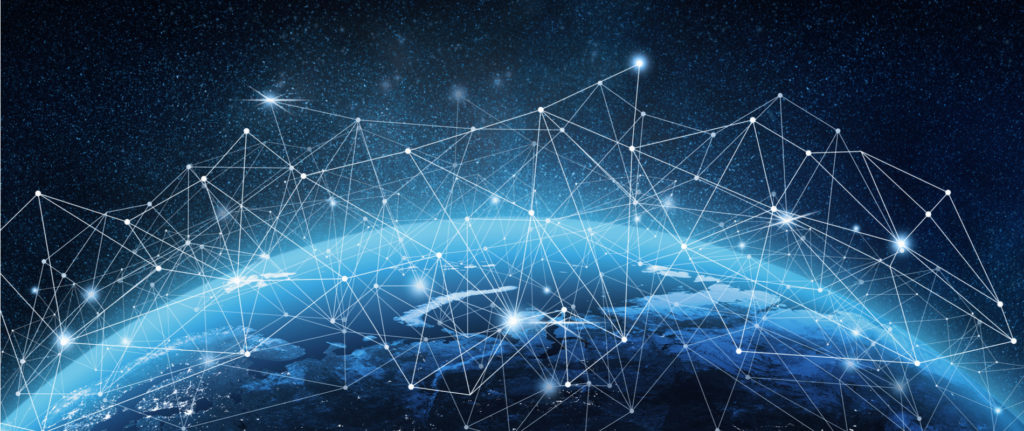
\includegraphics[width=15cm]{redes.jpg}
    \vfill
    \vfill
\end{titlepage}

\newpage
\tableofcontents
\newpage

\section{Sistemas de comunicación y redes}
\textbf{Sistema de comunicación:} infraestructura (hardware y software) que permite el intercambio de información. \\

\textbf{Información:} Conjunto de datos con significado. \\

\textbf{Red (de computadores, de móviles, de dispositivos \ldots):} sistema de comunicación con sistemas finales (terminales) autónomos (con capacidad de procesar información) que facilita el intercambio eficaz y transparente de información. \\

Entre las razones(motivaciones) para usar redes se encuentran, compartir recursos, escalabilidad, fiabilidad, robustez y ahorro de costes (computación distribuida). \\

Generalmente de una red se espera:

\begin{itemize}
\item Autonomía: capacidad de procesar información
\item Interconexión: mediante un sistema de comunicación
\item Intercambio de información, con eficacia y transpariencia´
\end{itemize}

\begin{figure}[h]
\centering
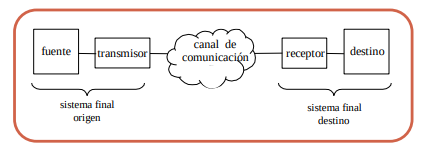
\includegraphics[scale=1,width=1\textwidth]{esquema_canal_comunicacion.png}
\caption{Esquema Canal de Comunicacion}
\end{figure}

\textbf{Estructura y elementos de una red:}
\begin{itemize}
\item Hosts: sistemas finales (terminales) autónomos.
\item Subred: infraestructura para el transporte de información (línea de transmisión, nodos o elementos de conmutación: routers / switches)
\end{itemize}

\textbf{Medios de transmisión:}

Dentro de los medios físicos de transmisión diferenciamos entre medios guiados y medios no guiados.

\begin{itemize}
\item \textbf{Medios guiados:} las ondas se canalizan a través de un medio sólido.
\item \textbf{Medios no guiados:} las ondas se propagan por la atmósfera y el espacio exterior, tal como ocurren en las redes LAN inalámbricas o en un canal de satélite digital.
\end{itemize}

\begin{itemize}
\item \textbf{Cable Coaxial:} posee dos conductores concéntricos, uno central, llamado núcleo, encargado de llevar la información, y uno exterior, de aspecto tubular, llamado malla, blindaje o trenza, que sirve como referencia de tierra y retorno de las corrientes. Entre ambos se encuentra una capa aislante dieléctrica, de cuyas características dependerá principalmente la calidad del cable. Todo el conjunto suele estar protegido por una cubierta aislante (también denominada camisa exterior).

\begin{figure}[h]
\centering
\caption{Ejemplo cable coaxial}
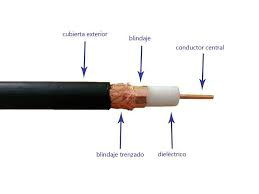
\includegraphics[scale=1,width=0.8\textwidth]{cable_coaxial.jpeg}
\end{figure}

\item \textbf{Cable de par trenzado:} tipo de cable que tiene dos conductores eléctricos aislados y entrelazados para anular las interferencias de fuentes externas y diafonía de los cables adyacentes. 
	\begin{itemize}
		\item \textbf{Unshielded twisted pair(UTP):} contiene pares trenzados sin blindar que se utilizan para diferentes tecnoloǵias de redes locales. Son de bajo costo y fácil uso, pero produce más errores que otros tipos de cables y tiene limitaciones para trabajar a grandes distancias sin regeneración de señal.
		
		\begin{figure}[h]
		\centering
		\caption{Ejemplo cable de par trenzado UTP}
		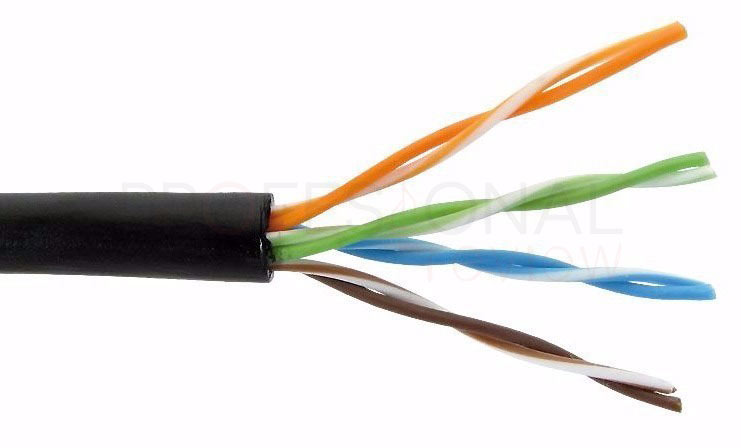
\includegraphics[scale=1,width=0.8\textwidth]{ejemplo_cable_utp.jpg}
		\end{figure}
		
		\item \textbf{Shielded twisted pair(STP):} contiene pares trenzados rodeados cada par de una cubierta hecho de aluminio. Se utiliza en redes de ordenadores como ethernet o Token Ring.
		
		\begin{figure}[h]
		\centering
		\caption{Ejemplo cable de par trenzado STP}
		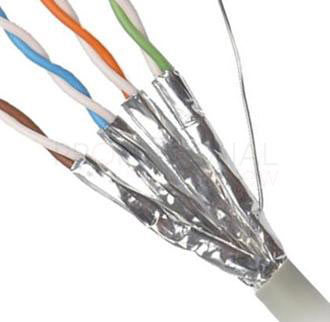
\includegraphics[scale=1,width=0.6\textwidth]{ejemplo_cable_stp.jpg}
		\end{figure}
		
		\item \textbf{Foiled twisted pair (FTP):} contiene pares trenzados, todos rodeados de una cubierta protectora hecha de alumino. Utilizado en equipo inalámbrios en exteriores.
		
		\begin{figure}[h]
		\centering
		\caption{Ejemplo cable de par trenzado FTP}
		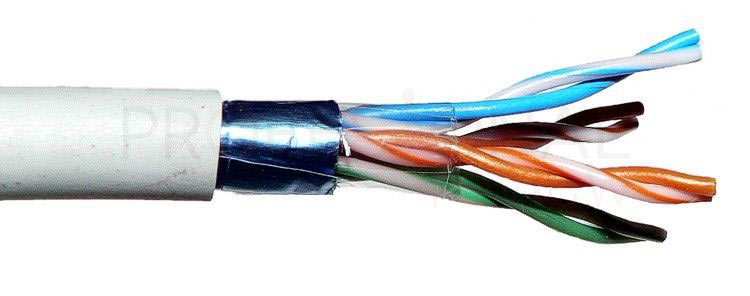
\includegraphics[scale=1,width=0.8\textwidth]{ejemplo_cable_ftp.jpg}
		\end{figure}
	\end{itemize}
	
\item \textbf{Fibra óptica:} fibra flexible, transparente, hecha al embutir o extruir vidirio o plástico en un diámetro ligeramente más grueso que el cabello humano. Se usan fibras en vez de alambre de metal porque las señales viajan a través de ellas con menos pérdida y además estas son inmunes a la interferencia electromagnética. FTTx (Fiber to the x) se origina como generalización de las distintas configuaraciones desplegadas, diferenciandose por la última letra que denota los distintos destinos de la fibra (nodo, acera, edificio, hogar \ldots).

\item \textbf{Canales de radio terrestres:} transportan señales dentro del espectro electromagnético, no requieren la instalación de cables físicos, pueden atravesar paredes, proporcionan conectividad a los usuarios móviles y potencialmetne pueden transportar una señal a grandes distancias.

\item \textbf{Canales de radio vía satélite:} un satélite de comunicaciones enlaza dos o más transmisores/receptores de microondas situados en la superficie, que se conocen como estaciones terrestres. El satélite recibe las transmisiones en una banda de frecuencia, regenera la señal utilizando un repetidor y transmite la señal a otra frecuencia. En este tipo de comunicaciones se emplean dos tipos de satélites: los satélites geoestacionarios y los satélites de la órbita baja terrestre (\textbf{LEO, Low-Earth Orbiting}).
\end{itemize}

\textbf{Topologías de redes:} patrón de interconexión entre sus nodos.
\begin{itemize}
\item \textbf{Topología física:} es una configuración de nodos y las conexiones físicas entre ellos. La representación de cómo se usan los medios para interconectar los dispositivos es la topología físcia.

\begin{figure}[h]
\centering
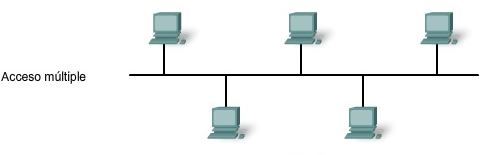
\includegraphics[scale=1,width=0.8\textwidth]{topologia_fisica.png}
\caption{Ejemplo Topologia Fisica}
\end{figure}

\item \textbf{Topología lógica:} es la forma en que una red transfiere tramas de un nodo al siguiente. Esta configuración consiste en conexiones virtuales entre los nodos de una red independientemente de su distribución física. Los protocolos de la capa de enlace de datos definen estas rutas de señales lógicas. La capa de enlace de datos "ve" la topología lógica de una red al controlar el acceso de datos a los medios. Es la topología lógica la que influye en el tipo de trama de red y control de acceso a los medios que se utilizan.

\begin{figure}[h]
\centering
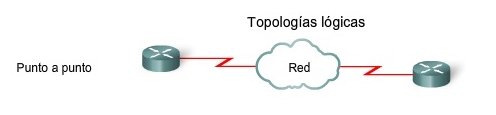
\includegraphics[scale=1,width=0.8\textwidth]{topologia_logica.png}
\caption{Ejemplo Topología Lógica}
\end{figure}

\end{itemize}

Tipos de topologías fisicas de redes:

\begin{itemize}
\item En bus: se caracteriza por tener un único canal de comunicaciones (denominado bus, torncal o backbone) al cual se conectan los diferentes dispositivos. De esta forma todos los dispositivos comparten el mismo canal.

	\begin{itemize}
		\item \textbf{Ventajas:} facilidad de implementación, fácil adaptación, simplicidad en la arquitectura y no ocupa mucho espacio.
		\item \textbf{Desventajas:} hay un límite de equipos dependiendo de la calidad de la señal, puede producirse degradación de la señal, complejidad de reconfiguración y asilamiento de fallos, limitación de las longitudes físicas del canal, un problema en el canal usualmente degrada toda la red, el desempeño se disminuye a medida que la red crece, el canal requiere ser correctamente cerrado y altas pérdidas en la transmisión debido a colisiones entre mensajes.
	\end{itemize}
	
	\begin{figure}[h]
		\centering
		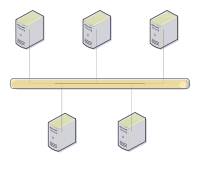
\includegraphics[scale=1,width=0.6\textwidth]{topologia_bus.png}
		\caption{Red en Bus}
	\end{figure}
	
\item En anillo: topología de red en la que cada nodo se conecta exactamente a otros dos nodos, formando una única ruta continua, para las señales a través de cada nodo, es decir, un anillo. Los datos viajan de un nodo a otro, y cada nodo maneja cada paquete.

	\begin{itemize}
		\item \textbf{Ventajas:} red muy ordenada donde cada dispositivo tiene acceso al token y la oportunidad de transmitir. Se desempeña mejor que una topología de bus bajo una gran carga de red, además, no requiere un nodo central para administrar la conectividad entre las computadoras, debido a la configuración de línea de punto a punto de los dispositivos con un dispositivo a cada lado, que es bastante fácil de instalar y reconfigurar, ya que agregar o quitar un dispositivo requiere mover solo dos conexiones. La configuración de línea punto a punto facilita la identificación y el aislamiento de fallas y la reconfiguración de las fallas de línea de los anillos bidireccionales puede ser muy rápida, ya que la conmutación se produce en un nivel alto y, por lo tanto, el tráfico no requiere ser redirigido individualmente.
		
		\item \textbf{Desventajas:} una estación de trabajo defectuosa puede crear problemas para toda la red, mover, agregar y cambiar los dispositivos puede afectar a la red, el retraso en la comunicación es directamente proporcional al número de nodos en la caja de cambios, el ancho de banda se comparte en todos los enlaces entre dispositivos y es más difícil de configurar que una topología en estrella.
	\end{itemize}
	
	\begin{figure}[h]
		\centering
		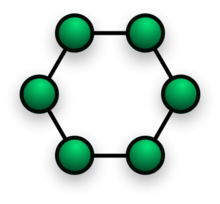
\includegraphics[scale=1,width=0.6\textwidth]{topologia_anillo.png}
		\caption{Red en Anillo}
	\end{figure}

\item En estrella:  red de computadoras donde las estaciones están conectadas directamente a un punto central y todas las comunicaciones se hacen necesariamente a través de ese punto (conmutador, repetidor o concentrador). Los dispositivos no están directamente conectados entre sí, además de que no se permite tanto tráfico de información. Dada su transmisión, una red en estrella activa tiene un nodo central activo que normalmente tiene los medios para prevenir problemas relacionados con el eco.

	\begin{itemize}
		\item \textbf{Ventajas:} posee un sistema que permite agregar nuevos equipos fácilmente, reconfiguración rápida, fácil de prevenir daños y/o conflictos, ya que no afecta a los demás equipos si ocurre algún fallo, centralización de la red y fácil de encontrar fallas de cada uno de ellos.
	
		\item \textbf{Desventajas:} si el hub(repetidor) o switch central falla, toda la red deja de transmitir, es costosa, ya que requier más cables que otras topologías y el cable viaja por separado del concentrador a cada computadora.
	\end{itemize}
	
	\begin{figure}
		\centering
		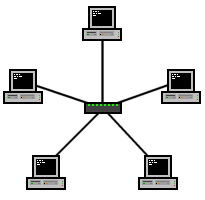
\includegraphics[scale=1,width=0.6\textwidth]{topologia_estrella.png}
		\caption{Red en Estrella}
	\end{figure}
	
\item En árbol: es una topología de red en la que los nodos están colocados en forma de árbol. Desde una visión topológica, es parecida a una serie de redes en estrella interconectadas salvo en que no tiene un concentrador central. En cambio, tiene un nodo de enlace troncal, generalmente ocupado por un hub o switch, desde el que se ramifican los demás nodos. Es una variación de la red en bus, el fallo de un nodo no implica una interrupción en las comunicaciones. Se comparte el mismo canal de comunicaciones.

	\begin{itemize}
		\item \textbf{Ventajas:} cableado punto a punto para segmentos individuales, soportado por multitud de vendedores de software y de hardware, facilidad de resolución de problemas y mucho más rápida que otra.
		
		\item \textbf{Desventajas:} Se requiere mucho cable, es poco fiable para las empresas distribuidas, la medida de cada segmento viene determinada por el tipo de cable utilizado, si se cae el segmento principal todo el segmento cae, es más difícil de configurar y si se llegara  a desconectar un nodo, todos los que están conectados a él se desconectan también.
	
	\end{itemize}
	
	\begin{figure}[h]
		\centering
		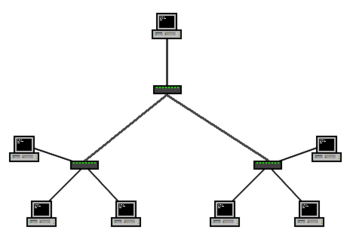
\includegraphics[scale=1,width=0.7\textwidth]{topologia_arbol.png}
		\caption{Red en Árbol}
	\end{figure}
	
\item Mallada: es una topología de red en la que cada nodo está conectado a todos los nodos. De esta manera es posible llevar los mensajes de un nodo a otro por distintos caminos. Si la red de malla está completamente conectada, no puede existir absolutamente ninguna interrupción en las comunicaciones. Cada servidor tiene sus propias conexiones con todos los demás servidores.

	\begin{itemize}
		\item \textbf{Ventajas:} es posible llevar los mensajes de un nodo a otro por diferentes caminos, no puede existir absolutamente ninguna interrupción en las comunicaciones, cada servidor tiene sus propias comunicaciones con todos los demás servidores, si falla un cable el otro se hará cargo del tráfico, no requiere un nodo o servidor central lo que reduce el mantenimiento, si un nodo desaparece o falla no afecta en absoluto a los demás nodos y si desaparece no afecta tanto a los nodos de redes.
		
		\item \textbf{Desventajas:} el costo de la red puede aumentar en los casos en los que se implemente de forma alámbrica. La  topología de red y las características de la misma implican el uso de más recursos, la disponibilidad del ancho de banda puede verse afectada por la cantidad de usuarios que hacen uso de la red simultánemanete, para entregar un ancho de banda que garantice la tasa de datos en demanda y, que en particular, garantice las comunicaciones , es necesario instalar más puntos de acceso, por tanto, se incrementan los costos de implementación y puesta en marcha.
	\end{itemize}
	
	\begin{figure}
		\centering
		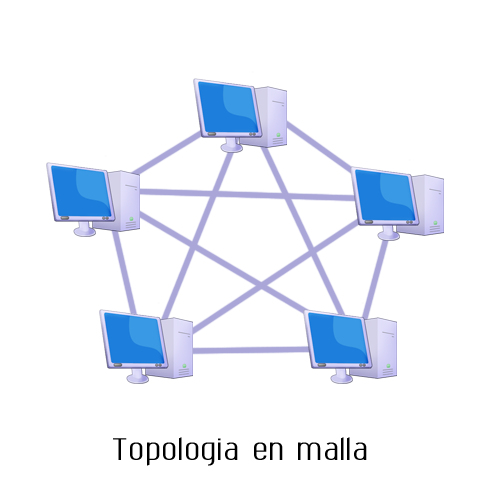
\includegraphics[scale=1,width=0.6\textwidth]{topologia_malla.png}
		\caption{Red en Malla}
	\end{figure}

\item Híbrida: en este tipo de topología las redes pueden utilizar diversas topologías para conectarse. La topología mixta es una de las más frecuentes y se deriva de la unión de varios tipos de topologías de red, de aquí el nombre de mixtas o híbridas.
\end{itemize}

Clasificación de redes:

\begin{itemize}
\item Según tamaño y extensión:
	\begin{itemize}
		\item \textbf{Personal Area Network(PAN)}: es un estándar de red para la comunicación entre distintos dispositivos cercanos al punto de acceso. Estas redes son de unos pocos metros y para uso personal.
		
		\item \textbf{Local Area Network (LAN):} es una red de computadoras que abarca un área reducida en una casa, un departamento o un edificio.
		
		\item \textbf{Metropolitan Area Network (MAN):} es una red de alta velocidad (banda ancha) que da cobertura geográfica extensa, proporcionando capacidad de integración de múltiples servicios mediante la transmisión de datos, voz y vídeo, sobre medios de transmisión tales como fibra óptica y par trenzado.
		
		\item \textbf{Wide Area Network (WAN):} es una red de computadoras que une varias redes locales, aunque sus miembros no estén todos en una misma ubicación física. Muchas WAN son construidas por organizaciones o empresas para su uso privado, otras son instaladas por los proveedores de Internet (ISP) para proveer conexión a sus clientes.
	\end{itemize}
	
\item Según tecnología de transmisión:
	
	\begin{itemize}
		\item \textbf{Difusión:} en las redes broadcast hay un único canal de comunicación, compartido por todos los ordenadores de la red. Los ordenadores envían mensajes cortos, denominados tramas, que llegan al resto de los ordenadores de la red. Sin embargo, esto no quiere decir que todos los mensajes tengan como destinatarios, siempre, la totalidad de los ordenadores de la red.
		
		\item \textbf{Punto a Punto:} las conexiones son punto a punto entre pares de ordenadores. Se establece una comunicación directa entre los dos ordenadores. Hasta que un mensaje no llega a su destino, puede pasar por varios nodos intermedios. Dado que normalmente, existe más de un camino posible, hay algoritmos de encaminamiento (routing), que lo gobiernan.
	\end{itemize}
	
\item Según el tipo de transferencia de datos:
	
	\begin{itemize}
		\item \textbf{Simplex:}  en esta redes los canles de comunicación manda información en una sola dirección.
		
		\begin{figure}[h]
			\centering
			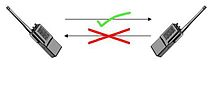
\includegraphics[scale=1,width=0.6\textwidth]{simplex.jpg}
			\caption{Conexión Simplex}
		\end{figure}
		
		\item \textbf{Half-Duplex:} en estas conexiones los datos fluyen en una o en otra dierección pero no en las dos direcciones al mismo tiempo. Con este tipo de conexión, cada extremo de la conexión transmite uno después del otro.
		
		\begin{figure}[h]
			\centering
			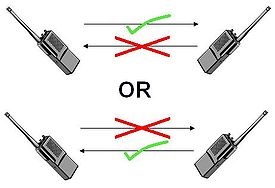
\includegraphics[scale=1,width=0.6\textwidth]{half_duplex.jpeg}
			\caption{Conexión Half-Duplex}
		\end{figure}
		
		
		\item \textbf{Duplex:} estas conexiones permiten el envío y la recepción simultáneos de información.
		
		\begin{figure}[h]
			\centering
			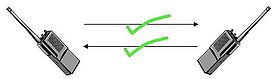
\includegraphics[scale=1,width=0.8\textwidth]{duplex.jpeg}
			\caption{Conexión Duplex}
		\end{figure}
	\end{itemize}
\end{itemize}


\section{Diseño y estandarización de redes:}
Estándares internacionales:

\begin{itemize}
\item \textbf{Modelo OSI (Open System Interconnection) de la ISO.}
\item \textbf{TCP/IP del Internet Engineering Task Force.}
\end{itemize}

\textbf{TCP/IP:} es una descripción de protocolos de red. Este modelo es usado para comunicación de redes y describe un conjunto de guías generales de operación para permitir que un equipo pueda comunicarse en una red. Provee conectividad de extremo a extremo especificando cómo los datos deberían ser formateados, direccionados, transmitidos, enrutados y recibidos por el destinatario. Este modelo y los protocolos relacionados son mantenidos por la Internet Engineering Task Force. \\

\begin{itemize}
\item \textbf{Capa de aplicación:} es dónde residen las aplicaciones de red y sus protocolos de nivel de aplicación. Esta incluye muchos protocolos tales como, HTTP (Hipertext Transfer Protocol: permite la solicitud y transferncia de documentos web), SMTP (Simple Mail Transfer Protocol: permite la transferencia de mensajes de correo electrónico) y FTP (File Transfer Protocol: permite la transferencia de archivos entre dos sistemas terminales). Un protocolo de la capa de aplicación está distribuido entre varios sistemas terminales, con la aplicación en un sistema terminal utilizando el protocolo para intercambiar paquetes de información con la aplicación que se ejecuta en otro sistema terminal. A este paquete de información se llama mensaje.

\item \textbf{Capa de transporte:} transporta los mensajes de la capa de aplicación entre los puntos terminales de la aplicación. En Internet, existen dos protocolos de transporte, TCP y UDP, pudiendo cada uno de ellos transportar los mensajes de la capa de aplicación. TCP (Transmission Control Protocol) ofrece a sus aplicaciones un servicio orientado a conexión. Este servicio incluye el suministro garantizado de los mensajes de la capa de aplicación al destino y un mecanismo de control de flujo. TCP también divide los mensajes largos en segmentos más cortos y proporciona un mecanismo de control de congestión , de manera que un emisor regula su velocidad de transmisión cuando la red está congestionada. UDP (User Datagram Protocol) proporciona a sus aplicaciones un servicio sin conexión. Es un servicio básico que no ofrece ninguna fiabilidad, ni control de flujo, ni control de gestión. Los paquetes de esta capa se denominan segmentos.

\item \textbf{Capa de red:} es responsable de trasladar los paquetes de la capa de red, conocidos como datagramas, de un host a otro. El protocolo de la capa de transporte (TCP o UDP) de un host origen pasa un segmento de la capa de transporte y una dirección de destino a la capa de red. La capa de red proporciona el servicio de suministrar el segmento a la capa de transporte del host de destino. Esta capa incluye el protocolo IP, que define los campos del datagrama, así como la forma en que actúan los sistemas terminales y los routers sobre estos campos. Existe un único protocolo IP y todos los componentes de Internet que tienen capa de red deben ejecutar el protocolo IP. Esta capa incluye protocolos de enrutamiento, que determinan las rutas que los datagramas siguen entre los orígenes y los destinos. 

\item \textbf{Capa de enlace:} para tasladar un paquete desde un nodo (host o router) al siguiente nodo de la ruta, la capa de red confía en los servicios de la capa de enlace. En cada nodo la capa de red pasa el datagrama a la capa de enlace, que entrega el datagrama al siguiente nodo existente a lo largo de la ruta. En ese siguiente nodo, la capa de enlace pasa el datagrama a la capa de red. Los servicios proporcionados por la capa de enlace dependen del protocolo que se emplee en el enlace. En esta capa se incluyen protocolos como Ethernet, WiFi y el protocolo DOCSIS de la red de acceso por cable. Puesto que un datagrama puede necesitar atravesar varios enlaces, puede ser manipulado por distintos protocolos de la capa de enlace en los distintos enlaces disponibles a los largo de la ruta. A los paquetes de esta capa los llamamos tramas.

\item \textbf{Capa física:} el trabajo de la capa física consiste en mover de un nodo al siguiente los bits individuales que forman la trama. Los protocolos de esta capa son, de nuevo, dependientes del enlace y, por tanto, depende del medio de transmisión del enlace.
\end{itemize}

\textbf{Modelo OSI (Open Systems Interconnection):} es un modelo de referncia para los protocolos de la red, creado en 1980 por la Organización Internacional de Normalización. Es un estándar que tiene por objetivo conseguir interconectar sistemas de procedencia distinta para que estos pudieran intercambiar información sin ningún tipo de impedimentos debido a los protocolos con los que estos operaban de forma propia según su fabricante.

\begin{figure}[h]
\centering
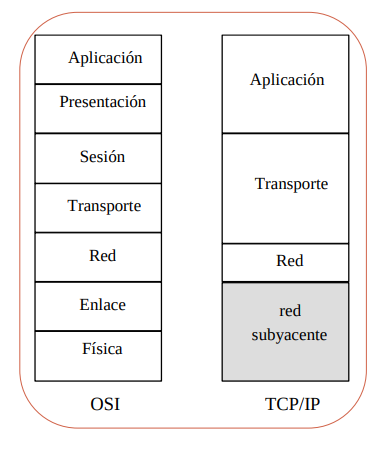
\includegraphics[scale=1,width=0.8\textwidth]{modelo_osi.png}
\end{figure}

\begin{itemize}
\item \textbf{Capa de aplicación:} ofrece a las aplicaciones la posibilidad de acceder a los servicios de las demás capas y define los protocolos que utilizan las palicaciones para intercambiar datos, como correo electrónico, SGBD y servidor de ficheros. Hay tantos protocolos como aplicaciones distintas y puesto que continuamente se desarrollan nuevas aplicaciones el número de protocolos crece sin parar. \\
Cabe aclarar que el usuario normalmente no interactúa directamente con el nivel de aplicación. Suele interactuar con programas que a su vez interactúan con el nivel de aplicación pero ocultando la complejidad subyacente.

\item \textbf{Capa de presentación:} el objetivo es encargarse de la representación de la información, de manera que, aunque distintos equipos puedan tener diferentes representaciones internas de caracteres, los datos lleguen de manera reconocible. Esta capa es la primera en trabajar más el contenido de la comunicación que el cómo se establece la misma. En ella se tratan aspectos tales como la semántica y la sintaxis de los datos transmitidos, ya que distintas computadoras pueden tener diferentes formas de manejarlas. Esta capa también permite cifrar los datos y comprimirlos. Por lo tanto, podría decirse que esta capa actúa como un traductor. Proporciona servicios que permitan a las  aplicaciones que se comunican interpretar el significado de los datos intercambiados. Estos servicios incluyen la comprensión y el cifrado de los datos (funciones cuyos nombres son autoexplicativos), así como la descripción de los datos (lo que libera a la apliación de tener que preocuparse por el formato interno en el que los datos se representan y almacenan, formatos que pueden diferir de una computadora a otra).

\item \textbf{Capa de sesión:} esta capa se encarga de mantener y controlar el enlace establecido entre dos computadores que están transmitiendo datos de cualquier índole. Por lo tanto, el servicio provisto por esta capa es la capacidad de asegurar que, dada una sesión establecida entre dos máquinas, la misma se pueda efectuar para las operaciones definidas de principio a fin, reanudándolas en caso de interrupción. En muchos casos, los servicios de la capa de sesión son parcial o totalmente prescindibles. Permite delimitar y sincronizar el intercambio de datos, incluyendo los medios para crear un punto de restauración y un esquema de recuperación.

\item \textbf{Capa de transporte:} es la capa encargada de efectuar el trasporte de los datos de la máquina origen a la de destino, independientemente del tipo de red física que esté utilizando. La PDU (Protocol Data Unit) de la capa de transporte se llama Segmento o Datagrama, dependiendo de si corresponde a TCP (Transmission Control Protocol) o UDP (User Datagram Protocol), el primero orientado a conexión y el otro sin conexión. Trabajan, por lo tanto, con puertos lógicos y junto con la capa red dan forma a los conocidos como Sockets IP:Puerto.

\item \textbf{Capa de red:} se encarga de identificar el enrutamiento existente entre una o más redes. Las unidades de datos se denominan paquetes, y se pueden clasificar en protocolos enrutables y protocolos de enrutamiento. 

	\begin{itemize}
		\item Enrutables: viajan con los paquetes (IP,IPX,APPLETALK)
		\item Enrutamiento: permiten seleccionar las rutas (RIP,IGRP,EIGRP, \newline OSPF,BGP)
	\end{itemize}

El objetivo de esta capa es hacer que los datos lleguen desde el origen al destino, aun cuando ambos no estén conectados directamente sino que utilicen dispositivos intermedios. Los dispositivos que facilitan tal tarea se denominan encaminadores o enrutadores. Estos trabajan en esta capa, aunque pueden actuar como switches de nivel 2 en determiandos casos, dependiendo de la función que se le asigne. Los firewalls actúan sobre esta capa principalmente, para descartar direcciones de determinadas máquinas o limitar el acceso a ciertas de ellas. En este nivel se realiza el direccionamiento lógico y la determinación de la ruta de los datos hasta su receptor final. A menudo la implementación de esta capa es mixta de hardware y software.

\item \textbf{Capa de enlace de datos:} Esta capa se ocupa del direccionamiento físico, del acceso al medio, de la detección de errores, de la distribución ordenada de tramas y del control del flujo. \\

Es uno de los aspectos más importantes que revisar en el momento de conectar los ordenadores, ya que está entre la capa 1 y 3 como parte esencial para la creación de sus protocolos básicos (MAC, IP), para regular la forma de la conexión entre computadoras, determinando el paso de tramas, verificando su integridad, y corrigiendo erroes. Por lo cual es importante mantener una excelente adecuación al medio físico, con el medio de red que redirige las conexiones mediante un enrutador. \\

Dadas estas situaciones cabe recalcar que el dispositivo que usa la capa de enlace es el Switch que se encarga de recibir los datos del enrutador y enviar cada uno de estos a sus respectivos destinatarios, dada esta situación se determina como el medio que se encarga de la corrección de errores, manejo de tramas, protocolización de datos (se llaman protocolos a las 'reglas de cortesía' o convenciones que debe seguir cualquier capa del modelo OSI). Las capas de enlace y física normalmente se implementan en las tarjetas de interfaz de red asociadas a un determinado enlace.

\item \textbf{Capa física:} es la que se encarga de la topología de red y de las conexiones globales de la computadora hacia la red, se refiere tanto al medio físico como a la forma en la que se transmite la información y de las redes. Sus principales funciones son:

	\begin{itemize}
		\item Definir el medio o medios físicos por los que va a viajar la comunicación.
		\item Definir las característica materiales y eléctricas que se van a usar en la transmisión de los datos por los medios físicos.
		\item Definir las características funcionales de la interfaz.
		\item Transmitir el flujo de bits a través del medio.
		\item Manejar las señales eléctricas del medio de transmisión, polos en un enchufe, etc.
		\item Grantizar la conexión (aunque no la fiabilidad de dicha conexión).
	\end{itemize}

 
\end{itemize}

\section{Terminología, conceptos y servicios.}
Retardos en la comunicación. \\
(1)Transmisión $\rightarrow T_t=L(bits)/V_t(bps)$ \\
(2)Propagación $\rightarrow T_p=D(m)/V_p(m/s)$ \\
(3)Procesamiento(interno) + retardo en la cola + acceso al medio. \\

,donde ($L(bits)$=longitud del paquete en bits, $V_t$=velocidad de transmisión en bit por segundo, $D(m)$= distancia en metros que separan los terminales y $V_p$= velocidad de propagación. \\

Tipos de retardo más importantes:
\begin{itemize}
\item \textbf{Retardo de procesamiento:} tiempo requerido para examinar la cabecera del paquete y determinar dónde hay que enviarlo. Este retardo puede incluir otros factores, como el tiempo necesario para comprobar los errores de nivel de bit del paquete que se hayan producido al transmitir los bits del paquete.

\item \textbf{Retardo de cola:} tiempo que el paquete espera para ser transmitido a través del enlace. Dependerá del número de paquetes que hayan llegado antes a la cola y que estén esperando para ser transmitidos por el enlace. 

\item \textbf{Retardo de transmisión:} tiempo necesario para introducir todos los bits del paquete en el enlace.

\item \textbf{Retardo de propagación:} tiempo necesario para propagar un paquete desde el principio del enlace hasta el final del mismo, es decir, hasta su destino.

\item \textbf{Pérdida de paquetes:} se dice que un paquete se pierde cuando este llega a un router y se encuentra conque la cola del mismo está llena, con lo que el router elimina este paquete.

\end{itemize}

Tipos de servicios:

\begin{itemize}
\item \textbf{Orientado a conexión(SOC):} en estos servicios se debe establecer una conexión antes de transferir datos. Se identifica el flujo de tráfico con un identificador de conexión en lugar de utilizar explícitamente las direcciones de la fuente y el destino.

\item \textbf{No orientado a conexión (SNOC):} una comunicación entre dos puntos finales de una red en los que un mensaje puede ser enviado desde un punto final a otro sin acuerdo previo. El dispositivo en un extremo de la comunicación transmite los datos al otro, sin tener que asegurarse de que el receptor esté disponible y listo para recibir los datos. El emisor simplemente envía un mensaje dirigido al receptor.
\end{itemize}

Además destacar, que dentro de estos a se puede tener una conexión en la que los terminales confirman la recepción de un paquete con el envío de un ACK al origen de dicho envío.

\section{Internet: topología y direccionamiento.}
\textbf{Historia de Internet:}
\begin{itemize}
\item 70s: DARPA inicia proyecto en redes con dos objetivos básicos:
	\begin{itemize}
		\item Robustez en las comunicaciones.
		\item Seguridad en las transmisiones.
	\end{itemize}
	
\item 1973: Metcalfe inventa Ethernet (tesis doctoral).
\item 80s: La red creada se divide en dos.
 	\begin{itemize}
 		\item ARPANET.
 		\item MILNET.
 	\end{itemize}
 	
\item 1983: Aparece el S.O. UNIX de BSD (Universidad de Berkeley), que incluye:

	\begin{itemize}
		\item Nuevos protocolos: TCP/IP, el servicio de nombres DNS.
		\item Utilidades de servicios de red.
		\item La API socket.
	\end{itemize}

Se crea el IAB (Internet Architecture Board) dependiente del Department of Defense.

\item 1986: Aparece una nueva red troncal: NSFNET, motor impulsor de la actual Internet.
\item 1989: Tim Berners Lee(CERN) crear el intercambio de hipertextos (HTTP,HTMIL). La IAB se independiza y se organiza en dos grupos.
	
		\begin{itemize}
			\item IRTF (Internet Research Task Force).
			\item IETF (Internet Engineering Task Force)
		\end{itemize}
\item 1993: Primer navegador con interfaz gráfica (GUI): MOSAIC.
\item 1996: Microsoft incorpora el "explorer" dentro del S.O.
\end{itemize}

\textbf{Topología jerárquica}, niveles:

\begin{itemize}
\item Intranets (Ethernet-WiFi) del usuario: zona pública + zona privada
\item Redes de acceso (xDSL, RDSI, FTTH, etc) del Internet Service Provider (ISP).
\item Redes troncales (ATM, SDH, SONET,MPLS) de grandes operadores de telecomunicaciones.
\item Acuerdos de Peering y Tránsito.
\item Tier 1, Tier 2 y Tier 3.
\item Puntos neutros ó PoP (Point of Presence) ó IXP (Internet eXchange Point).
\end{itemize}

\textbf{Distintos niveles de redes:}
\begin{itemize}
\item \textbf{Redes Tier 1}: de grandes operadores globales, al menos en 2 continentes. Todas las redes Tier 1 están conectadas entre sí (backbone de Internet).
\item \textbf{Redes Tier 2}: de ámbito más regional, necesitan pasar por una red Tier 1 para llegar a toda Internet. Ofrecen servicios de conectividad a operadores Tier 3.
\item \textbf{Redes Tier 3}: operadores que dan servicio de conexión a Internet a usuarios y empresas (ISPs (Internet Service Providers)).
\end{itemize}

\textbf{Niveles de direccionamiento:}
\begin{itemize}
\item URL $\rightarrow$ capa de aplicación.
\item Puertos: identifica el proceso origen y destino $\rightarrow$ capa de transporte.
\item Dirección IP (identifica los hosts) $\rightarrow$ capa de red.
\end{itemize}



\section{Glosario}
\begin{itemize}
\item \textbf{Router:} dispositivo que permite interconectar computadoras que funcionan en el marco de una red. Se encarga de establecer la ruta que destinará a cada paquete de datos dentro de una red informática.

\item \textbf{Switches:}  dispositivo digital lógico de interconexión de equipos que opera en la capa de enlace de datos del modelo OSI. Su función es interconectar dos o más host de manera similar a lo puentes de red, pasando datos de un segmento a otro de acuerdo con la dirección MAC de destino de las tramas en la red y eliminando la conexión una vez finalizada esta.

\item \textbf{Puente de red:} es el dispositivo de interconexión de redes de computadoras que operan en el nivel de enlace del modelo OSI. Inteconecta segmentos de red (o divide una red en segmentos) haciendo la tranferencia de datos de una red hacia otra con base en la dirección física de destino de cada paquete.

\item \textbf{Dirección MAC (Media Access Control):} es un identificador de 48 bits (6 bloques de dos caracteres) que corresponde de forma única a una tarjeta o dispositivo de red. Se le conoce tamién como dirección física, y es única para cada dispositivo. 

\item \textbf{RFC (Request For Comments):} son un conjunto de documentos que sirve de referencia para la comunidad de internet, que describen, especifican y asisten en la implementación, estandarización y discusión de la mayoría de las normas, los estándares, las tecnologías y los protocolos relacionados con Internet y las redes en general. 

\item \textbf{SDU (Service Data Unit):} unidad de datos una vez derivada a la capa inferior en la pila de protocolos y que, una vez encapsulada por dicha capa, se convierte en la unidad de datos de protocolo de la misma.

\item \textbf{PDU (Protocol Data Unid):} especifica el conjunto de datos a enviar al protocolo par ubicado en el receptor.(Cabecera + SDU).

\item \textbf{SAP (Service Access Point):} es una etiqueta identificadora para endpoints de redes usados en redes que siguen el modelo OSI.

\item \textbf{Pila de Protolos (Protocol Stack):} es una colección ordenada de protocolos organizados en capas que se ponen unas encima de otras y en donde cada protocolo implementa una abstracción encuadrada en la abstracción que proporciona la capa sobre la que está encuadrada. Los protocolos en la capa inferior proporcionan sus servicios a los protocolos de la capa superior para que estos puedan realizar su propia funcionalidad.

\item \textbf{xDSL (x Digital Subscriber Line):} está formado por un conjunto de tecnología que proveen un gran ancho de banda sobre circuitos locales de cable de cobre, sin amplificadores ni repetidores de señal a lo largo de la ruta del cableado, entre la conexión del cliente y el primer nodo de la red. Un enlace DSL se comporta como tres enlaces separados, ya que en función de la frecuencia con la que se codifican datos y señales implican distintos canales.

\item \textbf{RDSI (Red Digital de Servicios Integrados):} red que procede por evolución de la Red Digital Integrada (RDI) y que facilita conexiones digitales extremo a extremo para proporcionar una amplia gama de servicios, tanto de voz como de otros tipos, y a la que los usuarios acceden a través de un conjunto de interfaces normalizados.

\item \textbf{Peering (conexión directa, intercambio de tráfico o emparejamiento)}: es la interconexión voluntaria de redes de Internet administrativamente independientes con el fin de intercambiar tráfico entre los usuarios de cada red. Las conexiones de peering se establecen sin restricciones y bajo un principio de libre acuerdo, en el que el cobro al usuario la realiza solo la operadora de la red de origen.

\item \textbf{PoP (Point of Presence):} es un lugar físico donde un proveedor de servicios tiene equipamiento, esto puede variar desde unos cuantos equipos, hasta pisos enteros de dispositivos. También se puede identificar como un punto de interconexión entre las instalaciones de comunicación suministradas por la empresa telefónica y la instalación de distribución principal del edificio.

\item \textbf{IXP (Internet eXchange Point):} infraestructura física a través de la cual los proveedores de servicios de internet intecambian el tráfico de internet entre sus redes. Esta instalación reduce la porción del tráfico de un ISP que debe ser entregado hacia su proveedor de conectividad, lo que reduce el costo promedio por bit de la entrega de su servicio. Además, el aumento del número de rutas aprendidas a través del punto neutro mejora la eficiencia de enrutamiento y la tolerancia de fallos.

\item \textbf{Interfaz de sockets:} es un cojunto de reglas que el programa que transmite los datos debe cumplir, para que internet pueda entregar esos datos al programa destino. 

\item \textbf{Protocolo:} define el formato y el orden de los mensajes intercambiados entre dos o más entidades que se comunican, así como las acciones tomadas al producirse la transmisión y/o recepción de un mensaje u otro suceso.

\item \textbf{DSLAM (Digital Subscriber Line Access Multiplexer):} es un multiplexor localizado dentro o fuera de la central telefónica que proporciona a los abonados o suscriptores el acceso a los servicios DSL sobre cable de par trenzado de cobre, separando la voz y los datos de las líneas de abonado.

\item \textbf{HFC (Hybrid Fiber Coax):} sistema por el cual el acceso por cable a internet utiliza la infraestructura de televisión por cable existente. Se usa fibra óptica para conectar el terminal de cabecera del cable a una serie de nodos de área situados en el vecindario, a partir de los cuales se utiliza cable coaxial tradicional para llegar a todos los domicilios.

\item \textbf{CMTS (Cable Modem Termination System):} equipo que se encuentra normalmente en la cabecera de la compañía de cable y se utiliza para proporcionar servicios de datos de alta velocidad, como internet por cable o voz sobre IP, a los abonados.

\item \textbf{PON (Passive Optical Network):} en estas cada vivienda dispone de una terminación de red óptica (ONT, Optical Network Terminator), que se conecta a un distribuidor del vecindario mediante un cable de fibra óptica dedicado. El distribuidor combina una cierta cantidad de viviendas en un único cable de fibra óptica compartido, que se conecta a una terminación de línea óptica (OLT, Optical Line Terminator) en la central de la compañía telefónica. La OLT, que realiza la conversión de señales ópticas en eléctricas, se conecta a Internet a través de un router de la compañía telefónica. En la arquitectura PON, todos los paquetes enviados desde la OTL al distribuidor se replican en este distribuidor.

\item \textbf{4G LTE (Long-Term Evolution):} tienes sus raíces en la tecnología 3G y puede conseguir velocidades superiores a 10Mbps. A diferencia del Wifi, un usuario solo necesita estar a unas pocas decenas de kilómetros de la estación base.

\item \textbf{Circuito:} en la jerga de la telefonía este término denomina a una conexión entre dos terminales que se mantiene durante toda la comunicación y en la que los recursos están reservados.

\item \textbf{FDM (Frequency-Division Multiplexing):} este tipo de multiplexación se utiliza para implementar los circuitos de un enlace. En esta el espectro de frecuencia de un enlace se reparte entre las conexiones establecidas a través del enlace. Específicamente el enlace dedica una banda de frecuencias a cada conexión durante el tiempo que esta dure.

\item \textbf{TDM (Time-Division Multiplexing):} este tipo de multiplexación también se usa para implementar los circuitos de un enlace. En este el tiempo se divide en marcos de duración fija y cada marco se divide en un número fijo de particiones. Cuando la red establece una conexión a través de un enlace, la red dedica una partición de cada marco a dicha conexión, y estas particiones están reservadas para uso exclusivo de dicha conexión, habiendo una partición disponible en cada marco para transmitir los datos de esa conexión.

\item \textbf{Modelo de servicio de una capa:} servicios que ofrece una capa a la capa que tiene por encima.

\item \textbf{Servicio orientado a conexión:} el usuario del servicio establece primero la conexión, la utiliza y después la termina. 

\item \textbf{Servicio sin conexión:} cada mensaje lleva consigo la dirección completa de destino y cada uno de ellos se encamina, de forma independiente, a través del sistema. Normalmente, cuando dos mensajes se envían al mismo destino, el primero que se envió será el primero en llegar, aunque es posible que el primero sufra un retardo y llegue el segundo. Esto es imposible en un servicio orientado a conexión. 

\item \textbf{Encapsulación:} el mensaje de una capa está encapsulado en el de la siguiente ya que cada capa añade información al mensaje. De aquí se deduce que cada capa está compuesta por un campo de cabecera y un campo de carga útil (normalmente es un paquete de la capa superior).

\item \textbf{Protocol fiable:} un protocolo se dice fiable si incorpora algún mecanismo que informe de si un datagrama ha sido entregado al extremo receptor con éxito o si no ha podido ser entregado. En caso contrario se dice no fiable.
\end{itemize} 





\end{document}